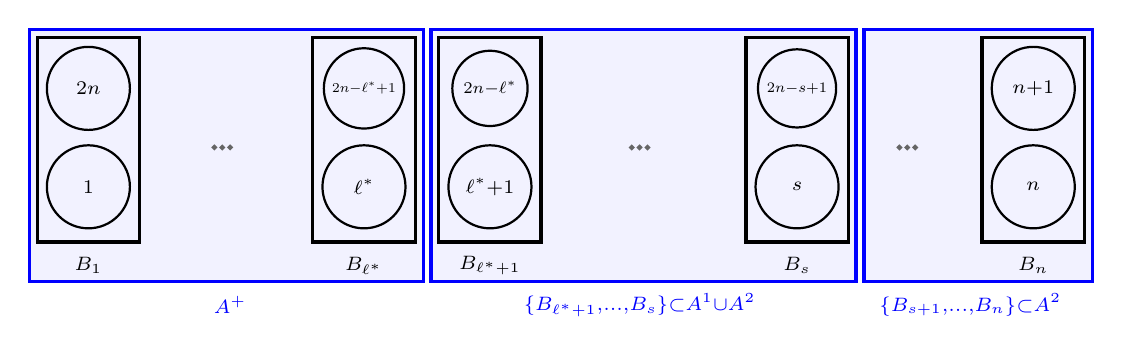
\begin{tikzpicture}
[scale=1,
 good/.style={circle, draw=black, thick, minimum size=30pt},
]

%A^+
\draw[blue, fill=blue!5, very thick] (-0.4-0.35,3.5) rectangle (0.26+4,0.3);
\node at (1.8, 0) {\textcolor{blue}{$\scriptstyle{A^+}$}};

%B_1
\draw[black, very thick] (-0.4-0.25,0.8) rectangle (0.4+0.25,3.4);

\node[good]      at (0,2.75)      {$\scriptstyle{2n}$};
\node[good]      at (0,1.5)      {$\scriptstyle{1}$};

\node at (0, 0.5) {$\scriptstyle{B_1}$};

%DOTS 
\filldraw[color=black!60, fill=black!5, thick](1.6, 2) circle (0.02);
\filldraw[color=black!60, fill=black!5, thick](1.7, 2) circle (0.02);
\filldraw[color=black!60, fill=black!5, thick](1.8, 2) circle (0.02);


%B_k
\draw[black, very thick] (-1.4-0.25 +4.5,0.8) rectangle (-0.6+0.25 +4.5,3.4);

\node[good, scale=0.7]      at (0 +3.5,2.75)      {$\scriptstyle{2n-\ell^*+1}$};
\node[good]      at (0 +3.5,1.5)      {$\scriptstyle{\ell^*}$};

\node at (0 +3.5, 0.5) {$\scriptstyle{B_{\ell^*}}$};

%A^1 \cup A^2
\draw[blue, fill=blue!5, very thick] (0.35+4,3.5) rectangle (4.75+5,0.3);
\node at (7, 0) {\textcolor{blue}{$\scriptstyle{\{B_{\ell^*+1}, \ldots, B_s\}\subset A^1 \cup A^2}$}};

%B_{k+1}
\draw[black, very thick] (-2.3-0.25 +7,0.8) rectangle (-1.5+0.25 +7,3.4);

\node[good,scale=0.85]      at (0 +5.1,2.75)      {$\scriptstyle{2n-\ell^*}$};
\node[good]      at (0 +5.1,1.5)      {$\scriptstyle{\ell^*+1}$};


\node at (0 +5.1, 0.5) {$\scriptstyle{B_{\ell^*+1}}$};

%DOTS 
\filldraw[color=black!60, fill=black!5, thick](2+4.9, 2) circle (0.02);
\filldraw[color=black!60, fill=black!5, thick](2.1+4.9, 2) circle (0.02);
\filldraw[color=black!60, fill=black!5, thick](2.2+4.9, 2) circle (0.02);

%B_{s}
\draw[black, very thick] (-3.4-0.25 +12,0.8) rectangle (-2.6+0.25 +12,3.4);

\node[good, scale=0.75]      at (0 +9,2.75)      {$\scriptstyle{2n-s+1}$};
\node[good]      at (0 +9,1.5)      {$\scriptstyle{s}$};

\node at (0 +9, 0.5) {$\scriptstyle{B_s}$};

%A^2
\draw[blue, fill=blue!5, very thick] (4.85+5,3.5) rectangle (7.75+5,0.3);
\node at (11.2, 0) {\textcolor{blue}{$\scriptstyle{\{B_{s+1}, \ldots, B_n\}\subset A^2}$}};

%DOTS 
\filldraw[color=black!60, fill=black!5, thick](5+5.3, 2) circle (0.02);
\filldraw[color=black!60, fill=black!5, thick](5.1+5.3, 2) circle (0.02);
\filldraw[color=black!60, fill=black!5, thick](5.2+5.3, 2) circle (0.02);

%B_{n}
\draw[black, very thick] (-0.4-0.25 +12,0.8) rectangle (0.4+0.25 +12,3.4);

\node[good]      at (0 +12,2.75)      {$\scriptstyle{n+1}$};
\node[good]      at (0 +12,1.5)      {$\scriptstyle{n}$};

\node at (0 +12, 0.5) {$\scriptstyle{B_n}$};

\end{tikzpicture}